\documentclass[12pt,letterpaper]{article}

\usepackage[utf8]{inputenc}
\usepackage[T1]{fontenc}
\usepackage[english]{babel}
\usepackage{float, enumitem, array, listings}
\usepackage{geometry, amsmath, amssymb, amsthm}
\usepackage{graphicx, xcolor, fancyhdr, fancyvrb}
\usepackage[normalem]{ulem}
\usepackage[hidelinks]{hyperref}

\geometry{margin=2cm, top=2cm, bottom=2cm}

\newcommand{\minic}{
  {M\footnotesize INI\normalsize C}
}

% ========================================
% CONSTANTES DEL ENCABEZADO
% ========================================
\newcommand{\encabezadoIzq}{Compiladores 2027-1}
\newcommand{\encabezadoCen}{Práctica 2}
\newcommand{\encabezadoDer}{\textit{Analizador léxico completo de \minic}}

% ========================================
% CONFIGURACION DEL ENCABEZADO
% ========================================
\pagestyle{fancy}
\fancyhf{}

\fancyhead[L]{\encabezadoIzq}
\fancyhead[C]{\encabezadoCen}
\fancyhead[R]{\encabezadoDer}

\fancyfoot[C]{\thepage}

\renewcommand{\headrulewidth}{0.1pt}
\renewcommand{\footrulewidth}{0pt}

% ========================================
% CONFIGURACION Y COLORES LSTLISTINGS
% ========================================
\renewcommand{\lstlistingname}{Código}

\definecolor{links}{HTML}{0D1894}

\definecolor{backcolour}{rgb}{0.93, 0.93, 0.93}
\definecolor{codegreen}{rgb}{0, 0.6, 0}
\definecolor{codegray}{rgb}{0.5, 0.5, 0.5}
\definecolor{codepurple}{rgb}{0.58, 0, 0.82}
\definecolor{keywordcolor}{rgb}{0.5, 0.0, 0.5}
\definecolor{codeorg}{HTML}{DB9400}
\definecolor{linkblue}{HTML}{1A167A}
\definecolor{redcolor}{HTML}{7A1805}
\definecolor{greencolor}{HTML}{0E8F10}
\definecolor{greeblucolor}{HTML}{0E6657}
\definecolor{orgcolor}{HTML}{B86D00}
\definecolor{highlightyellow}{HTML}{FFF176}
\definecolor{boxgray}{HTML}{F2F2F2}
\definecolor{borderblue}{HTML}{1A167A}

% ========================================
% CONFIGURACION LENGUAJES
% ========================================
\lstdefinestyle{modernc}{
    language=C,
    backgroundcolor=\color{backcolour},   
    commentstyle=\color{codegreen},
    keywordstyle=\color{keywordcolor}\bfseries,
    numberstyle=\tiny\color{codegray},
    stringstyle=\color{codepurple},
    basicstyle=\ttfamily\footnotesize,
    breakatwhitespace=false,
    breaklines=true,
    captionpos=b,
    keepspaces=true,
    numbers=left,
    numbersep=5pt,
    showspaces=false,                
    showstringspaces=false,
    showtabs=false,                  
    tabsize=4,
    frame=single,
    rulecolor=\color{black!20},
    frameround=tttt,
    emph={int,uint32_t,char,double,float,unsigned,void,bool,struct,size_t,
          Room, Client, pthread_mutex_t, NULL},
    emphstyle=\color{codeorg}\bfseries
}

\begin{document}

\thispagestyle{empty}
\begin{titlepage}
  \thispagestyle{empty}
  %--------------- COMANDO LINEA----------------->
  \newcommand{\linea}{\rule{\linewidth}{0.5mm}}                 
  \center
  %<<<<<<<<<<<<<<<<<<<<<<<<<<<<<<<<<<<<<<<<<<<

  %Add logos
  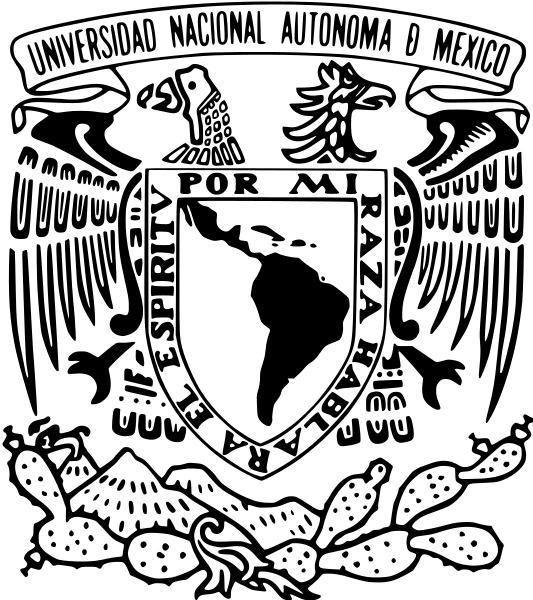
\includegraphics[width=0.24\textwidth]{../../unam_logo.png} \hspace{1.5cm}
  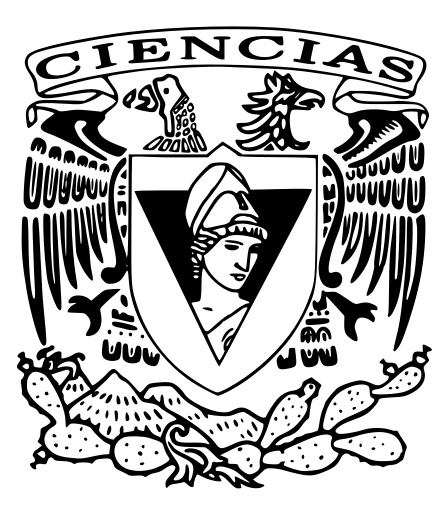
\includegraphics[width=0.25\textwidth]{../../fc_logo.png} \\[1cm]
  \textbf{\Large UNIVERSIDAD NACIONAL AUTÓNOMA}\\[3mm]
  \textbf{\Large DE MÉXICO} \\[6mm]
  \textit{\Large Facultad de Ciencias}

  \vfill

  %---------------TÍTULO----------------->
  \linea
  \vfill \vspace{1cm}
  \textbf{\Large Compiladores}\\[1.1cm]
  \textbf{\Large Analizador léxico completo de \minic}\\[0.9cm]
  \linea \\
  \vfill
  \vspace{0.7cm}
  %Title of the Research
  \textbf{\Large  Práctica 2}\\[6mm]
  %<<<<<<<<<<<<<<<<<<<<<<<<<<<<<<<<<<<<<<<<<<<

  %Team
  \vfill
  \textit{\small Presenta:}\\
  \textbf{\large  \textbf{Ramírez Juárez María Fernanda} - 321204747}\\[3mm]
  \textbf{\large  \textbf{Rojo Peña Manuel Ianluck} - 118005762}\\[3mm]

  %Profesor y Grupo
  \textit{\small Profesor:}\\
  \textbf{Pablo Martínez Yessica Janeth}\\[3mm]
  \textit{\small Ayudante de laboratorio:}\\
  \textbf{Salazar González Pedro Yamil}\\[3mm]
  \small Grupo: 7010, 2027-1\\[3mm]
  \vfill

  %Fecha or Date
  \textit{\small Fecha de entrega:}\\
         {\large 11 de septiembre, 2026}
         
\end{titlepage}


%%%%%%%%%%%%%%%%%%%%%%%%%%%%%%%%%%%%%%%%%%
\newpage
%%%%%%%%%%%%%%%%%%%%%%%%%%%%%%%%%%%%%%%%%%

% ================================================================
\section*{Objetivo}
% ================================================================

\begin{quote}
  En esta práctica nuestro objetivo fue extender el analizador léxico de \minic para que pudiera reconocer
  construcciones más complejas que un solo símbolo, puesto que, un lenguaje de programación se compone de mucho
  más que únicamente símbolos de un solo caracter como \texttt{=}, \texttt{+} o \texttt{;}, también se manejan
  operadores compuestos, palabras reservadas e identificadores.

  Concretamente, el objetivo es incorporar:
  
  \begin{enumerate}[label=\arabic*.]
  \item Conservar las funcionalidades ya implementadas en la Práctica 1
  \item Reconocer identificadores
  \item Distinguir entre identificadores, palabras reservadas (literales booleanos, condicionales)
  \item Reconocer operadores compuestos (\texttt{==}, \texttt{!=}, \texttt{<=}, \texttt{>=},
    \texttt{\&\&}, \texttt{||})
  \item Reconocer e ignorar comentarios de una línea
  \item Detectar caracteres no válidos y generarlos como \texttt{TOKEN\_ERROR} con su posición
  \item Recuperarnos  después de un error, sin detener la ejecución
  \item Generar correctamente el \texttt{TOKEN\_EOF} al final del archivo
  \end{enumerate}
  
  Además, tratamos de que el programa siguiera siendo robusto ante cadenas de longitud arbitraria
  (identificadores o enteros muy largos) y que el flujo de lectura del archivo se mantuviera claro y fácil
  de seguir. Al retomar la Práctica 1 notamos que, entre más casos añadíamos al ciclo principal, más difícil se
  volvía leer y de seguir, por lo que en esta práctica decidimos modularizar cada implementación de nuevo
  código en vez de simplemente apilar más condicionales por caso dentro del mismo ciclo.
\end{quote}


%%%%%%%%%%%%%%%%%%%%%%%%%%%%%%%%%%%%%%%%%%
\bigskip
%%%%%%%%%%%%%%%%%%%%%%%%%%%%%%%%%%%%%%%%%%


% ================================================================
\section*{Evolución respecto de la Práctica 1}
% ================================================================

Sin entrar mucho detalle, ya que lo describiremos más profundamente en la siguiente seccion, lo que hicismo
fue hacer la funcion \texttt{lexer\_scan} mucho más legible.

\subsection*{Módulos modificados o agregados}

\begin{itemize}
\item \texttt{lexer.h}: se agregó la estructura \texttt{Lexer}, que concentra todo el estado que antes
  manejábamos como variables y parámetros sueltos (\texttt{file}, \texttt{line}, \texttt{column}, \texttt{last\_was\_cr}, etc.), con un campo nuevo (\texttt{current}), que explicaremos más adelante, pero de manera rápida, nos indica el caracter actual.
\item \texttt{lexer.c}: se reescribió casi por completo, la función \texttt{simple\_token\_type} se convirtió en
  \texttt{scan\_simple} con un alcance más reducido, \texttt{advance\_position} se fusionó dentro de
  \texttt{lexer\_advance}, y se agregaron las funciones nuevas como \texttt{lexer\_init}, \texttt{lexer\_check},
  \texttt{emit\_token}, \texttt{scan\_operator}, \texttt{scan\_integer},
  \texttt{scan\_keyword} y \texttt{skip\_comment\_content}.
\item \texttt{keywords.h} y \texttt{keywords.c}: son un nuevo módulo, definimos la estructura \texttt{Keyword}
  y la función \texttt{lookup\_keyword}, que traduce un lexema a su \texttt{TokenType} si corresponde a una
  palabra reservada.
\item \texttt{buffer\_manage.h} y \texttt{buffer\_manage.c}: módulo nuevo, implementamos un buffer de texto
  dinámico (\texttt{TextBuffer}) que usamos para acumular lexemas de longitud variable no conocida de antemano
  (enteros, identificadores y palabras reservadas).
\end{itemize}

\subsection*{Cambios en la representación de tokens}

En la Práctica 1, solo emparejabamos los símbolos simples como \texttt{PLUS}, \texttt{MINUS}, \texttt{STAR},
\texttt{SLASH}, \texttt{ASSIGN}, \texttt{LESS}, \texttt{GREATER}, \texttt{LPAREN}, \texttt{RPAREN},
\texttt{LBRACE}, \texttt{RBRACE} y \texttt{SEMICOLON}; toknes de un solo caracter, sin distinguir todavía entre
un \texttt{=} suelto y un \texttt{==}, desarpovechando todos los demás tokens que en su enumeración ya venían
definidos como \texttt{EQUAL}, \texttt{NOT\_EQUAL}, \texttt{GREATER\_EQUAL}, etc.

\begin{lstlisting}[style=modernc, caption={Enumeración completa de \texttt{TokenType}, definida desde la Práctica 1 en \texttt{token.h}.}]
/* */
typedef enum {
    TOKEN_EOF,
    ERROR,
    IDENTIFIER,
    INTEGER,
    INT,
    BOOL,
    IF,
    ELSE,
    WHILE,
    PRINT,
    TRUE,
    FALSE,
    PLUS,
    MINUS,
    STAR,
    SLASH,
    ASSIGN,
    EQUAL,
    NOT_EQUAL,
    LESS,
    LESS_EQUAL,
    GREATER,
    GREATER_EQUAL,
    AND,
    OR,
    LPAREN,
    RPAREN,
    LBRACE,
    RBRACE,
    SEMICOLON
} TokenType;
\end{lstlisting}

\bigskip

Todos ellos se manejaban en lo que era la funcion \texttt{simple\_token\_type}, que ahora (sin entrar en mucho
detalle), la hemos refactorizado y cambiado el nombre a \texttt{scan\_simple}, donde ahora solo leemos los
caracteres que son únicamente simples, es decir que no pueden (al menos en este contexto de \minic) llegar a ser un operador compuesto:

\begin{lstlisting}[style=modernc, caption={\texttt{scan\_simple} de la Práctica 1 adaptado a las nuevas necesidades.}]
/* Escaneamos un caracter para verificar que tipo de simbolo simple es */
static int
scan_simple(int c,
            TokenType *type)
{
    if (type == NULL)
        return 0;
    
    switch (c) {
    case '+':
        *type = PLUS;
        break;
    case '-':
        *type = MINUS;
        break;
    case '*':
        *type = STAR;
        break;
    case '(':
        *type = LPAREN;
        break;
    case ')':
        *type = RPAREN;
        break;
    case '{':
        *type = LBRACE;
        break;
    case '}':
        *type = RBRACE;
        break;
    case ';':
        *type = SEMICOLON;
        break;
    default:
        return 0;
    }
    
    return 1;
}
\end{lstlisting}

\bigskip

Sigue sin ser la gran cosa, pues solo es un \texttt{switch} para emparejar el caso de cada simbolo con su token,
nótese que, como mencionamos, ya no están los casos para aquellps símbolos que pueden derivar en otros
operadores.

\subsection*{Correcciones efectuadas a la implementación anterior}

La corrección más relevante fue reemplazar el tamaño fijo del buffer que usábamos en la Práctica 1 para leer
enteros. En ese momento, por falta de tiempo, no retomamos la lógica de buffer dinámico que habíamos visto en
una de las primeras clases de laboratorio, y simplemente reservamos un arreglo de 64 bytes en la pila:

\begin{lstlisting}[style=modernc, caption={Buffer de tamaño fijo usado en la Práctica 1 (\texttt{lexer-p1.c}).}]
if (isdigit(c)) {
    char buffer[64];
    size_t len =  0;
    buffer[len++] = (char)c;

    int next;
    while ((next = fgetc(file)) != EOF && isdigit(next)) {
        if (len + 1 >= sizeof(buffer)) {
            fprintf(stderr, "Error: numero demasiado largo.\n ");
            return 2;
        }
        buffer[len++] = (char)next;
        advance_position(next, &line, &column, &last_was_cr);
    }
    buffer[len] = '\0';
    ...
}
\end{lstlisting}

\bigskip

Esto funcionaba para los casos de prueba de la Práctica 1, pero era una limitante considerable, un
identificador o un entero legítimo más largo de 63 caracteres haría fallar al programa con un error que no
tiene nada que ver con un error léxico real del programa fuente. En esta práctica sustituimos por completo
esta lógica por el módulo \texttt{buffer\_manage}, que describimos a detalle más adelante, y que tanto
\texttt{scan\_integer} como \texttt{scan\_keyword} reutilizan sin duplicar código entre sí.

\subsection*{Refactorizaciones relevantes y su justificación}

\begin{itemize}
\item \textbf{\texttt{simple\_token\_type} $\rightarrow$ \texttt{scan\_simple}.} Le quitamos los símbolos
  \texttt{=}, \texttt{<}, \texttt{>} y \texttt{/}, porque ahora estos pueden formar parte de un operador
  compuesto o de un comentario, y decidir eso requiere mirar el siguiente caracter antes de emitir un
  token. Dejar estos símbolos en \texttt{scan\_simple} habría significado alargar y añadir complejidad
  innecesaria a este función.
  
\item \textbf{\texttt{advance\_position} $\rightarrow$ \texttt{lexer\_advance}.} La función conserva la misma
  lógica de actualización de línea y columna, pero ahora es un método de la estructura \texttt{Lexer} y
  además es la única función responsable de leer un caracter nuevo del archivo. Esto evita que la
  actualización de posición y la lectura del archivo se hagan en dos lugares distintos (que fue,
  adelantando un poco, la causa de varios de los problemas que describimos en la sección de
  \nameref{sec:problemas}).
  
\item \textbf{\texttt{emit\_token} como función auxiliar nueva.} En la Práctica 1, el patrón
  \texttt{token\_init} \texttt{-} \texttt{token\_print} \texttt{-} \texttt{token\_destroy} se repetía en cada
  rama del \texttt{if}. Lo extrajimos a una sola función para que cada rama de \texttt{lexer\_scan} se reduzca a
  una sola línea, y para que un futuro cambio en cómo se emite un token (por ejemplo, un formato de
  salida distinto) solo tenga que ajustarse en un solo lugar.
  
\item \textbf{La estructura \texttt{Lexer} en sí misma.} Nuestra motivación principal era que las funciones
  auxiliares (\texttt{scan\_integer}, \texttt{scan\_keyword}, \texttt{scan\_operator}) necesitaban acceso
  al archivo y a la posición actual, y no queríamos pasarles cuatro parámetros sueltos a cada una (algo
  que sí hacíamos en un borrador intermedio). Agrupar todo en un solo \texttt{struct} y pasar un solo
  apuntador resuelve esto, y de paso deja espacio para el mecanismo de \textit{mirar-antes-de-consumir} que
  terminamos necesitando.
\end{itemize}


%%%%%%%%%%%%%%%%%%%%%%%%%%%%%%%%%%%%%%%%%%
\newpage
%%%%%%%%%%%%%%%%%%%%%%%%%%%%%%%%%%%%%%%%%%

% ================================================================
\section*{Descripción de la solución}
% ================================================================

Con \texttt{simple\_token\_type} ya reducida a \texttt{scan\_simple}, \texttt{lexer\_scan} queda mucho más
legible: se limita a mirar el primer caracter de cada posible token y delegar el resto de la lectura a una
función auxiliar según el caso.

\begin{lstlisting}[style=modernc, caption={La estructura \texttt{Lexer}, definida en \texttt{lexer.h}.}]
/* Estructura con la que podemos llevar un mejor flujo del proceso del lexer */
typedef struct {
    FILE *file;
    size_t line;
    size_t column;
    int last_was_cr;
    int current;
} Lexer;
\end{lstlisting}
\bigskip

Cada campo tiene un propósito concreto:

\begin{itemize}
\item \texttt{file}: el \texttt{FILE*} del que estamos leyendo, para no tener que pasarlo aparte a cada
  función auxiliar.
  
\item \texttt{line} / \texttt{column}: la posición actual dentro del archivo, por invariante de diseño,
  \texttt{line} y \texttt{column} siempre corresponden a la posición del caracter guardado en
  \texttt{current} (no a la del último caracter leído del disco, que puede ser distinto, como
  lo explicaremos más adelante).
  
\item \texttt{last\_was\_cr}: la bandera con la que recuerdamos si el caracter inmediatamente anterior fue un
  \texttt{\textbackslash r}. La necesitamos para tratar la secuencia \texttt{\textbackslash r\textbackslash n}
  como un único salto de línea, si ya contamos el salto de línea al procesar el \texttt{\textbackslash r},
  el \texttt{\textbackslash n} que le sigue no debe contarse una segunda vez.
  
\item \texttt{current}: el caracter que el lexer ya sacó del archivo pero que todavía no se ha consumido
  como parte de ningún token. Es la pieza que nos permite \emph{mirar} el siguiente caracter sin tener
  que procesarlo todavía, y es justo lo que necesitábamos para decidir, por ejemplo, si un
  \texttt{=} suelto es \texttt{ASSIGN} o el primer caracter de \texttt{EQUAL}.
\end{itemize}

\texttt{lexer\_init} deja el \texttt{Lexer} listo para empezar, precargando el primer caracter del archivo en
\texttt{current}:

\begin{lstlisting}[style=modernc, caption={Función \texttt{lexer\_init}.}]
/* Inicializamos la estructura lexer para empezar a leer el archivo */
static void
lexer_init(Lexer *lex,
           FILE *file)
{
    lex->file = file;
    lex->line = 1;
    lex->column = 0;
    lex->last_was_cr = 0;
    lex->current = fgetc(file);
}
\end{lstlisting}

\bigskip

\texttt{lexer\_check} simplemente devuelve ese caracter ya precargado, sin tocar el archivo ni la posición:

\begin{lstlisting}[style=modernc, caption={Función \texttt{lexer\_check}.}]
/* Devuelve el caracter aun no consumido, sin leer del archivo */
static int
lexer_check(Lexer *lex)
{
    return lex->current;
}
\end{lstlisting}

\bigskip

Y \texttt{lexer\_advance} es la única función que de verdad consume un caracter, toma lo que hay en
\texttt{current}, actualiza línea y columna según corresponda, y precarga en \texttt{current} el siguiente
caracter del archivo para que quede listo para la próxima llamada.

\begin{lstlisting}[style=modernc, caption={Función \texttt{lexer\_advance}.}]
/* Leemos un caracter del archivo y actualiza linea/columna segun corresponda */
static int
lexer_advance(Lexer *lex)
{
    int c = lexer_check(lex);
    
    if (c != EOF) {
        if (c == '\r'){
            (lex->line)++;
            lex->column = 0;
            lex->last_was_cr = 1;
        } else if (c == '\n') {
            if (lex->last_was_cr) {
                lex->last_was_cr = 0;
            } else {
                (lex->line)++;
                lex->column = 0;
            }
        } else {
            (lex->column)++;
            lex->last_was_cr = 0;
        }
        lex->current = fgetc(lex->file);
    }
    
    return c;
}
\end{lstlisting}
\bigskip

Con esto en mente y ya establecido, \texttt{lexer\_scan} queda así:

\begin{lstlisting}[style=modernc, caption={Función principal \texttt{lexer\_scan}.}]
/* Funcion principal que comienza el escaneo de un archivo para ser procesado por el lexer */
int
lexer_scan(FILE *file)
{
    int c;
    Lexer lex;

    if (file == NULL)
        return 2;

    lexer_init(&lex, file);
    
    while ((c = lexer_check(&lex)) != EOF) {
        size_t token_line = lex.line;
        size_t token_column = lex.column;
        TokenType type;

        lexer_advance(&lex);
                
        if (is_ignored_space(c))
            continue;

        //Comentarios
        if (c == '/') {
            if (lexer_check(&lex) == '/') {
                lexer_advance(&lex);
                skip_comment_content(&lex);
                continue;
            }
            if (!emit_token(SLASH, "/", token_line, token_column))
                return 2;
            continue;
        }

        //Operadores
        if (strchr("=<>!&|", c) != NULL) {
            char lexeme[3];
            type = scan_operator(&lex, c, lexeme);
            if (!emit_token(type, lexeme, token_line, token_column))
                return 2;
            continue;
        }

        //Numeros enteros
        if (isdigit(c)) {
            if (!scan_integer(&lex, c, token_line, token_column))
                return 2;
            continue;
        }
        
        //Identificadores y palabras reservadas
        if (isalpha(c) || c == '_') {
            if (!scan_keyword(&lex, c, token_line, token_column))
                return 2;
            continue;
        }
        
        //Simples
        if (scan_simple(c, &type)) {
            char lexeme[2] = {(char)c, '\0'};
            if (!emit_token(type, lexeme, token_line, token_column))
                return 2;
            continue;
        }        

        //Errores lexicos
        char lexeme[2] = {(char)c, '\0'};
         if (!emit_token(ERROR, lexeme, token_line, token_column))
             return 2;
    }

    if (ferror(file)) {
        fprintf(stderr, "Error: no se pudo leer el archivo.\n");
        return 2;
    }

    if (!emit_token(TOKEN_EOF, "", lex.line, lex.column))
        return 2;
    
    return 0;
}
\end{lstlisting}

\bigskip

Vale la pena que resaltemos el cambio en el ciclo principal, antes leíamos directamente con
\texttt{fgetc(file)} dentro de la condición del \texttt{while}, lo que quería decir que el caracter ya estaba
consumido en el momento en que entrábamos al cuerpo del ciclo. Ahora usamos \texttt{lexer\_check} para
\emph{mirar} el caracter (sin consumirlo todavía), guardamos \texttt{token\_line} y \texttt{token\_column} con
la posición correcta de ese caracter, y solo después llamamos a \texttt{lexer\_advance} para consumirlo de
verdad. Este orden de mirar, guardar posición, y hasta entonces consumir, es precisamente lo que terminamos
necesitando para que la posición reportada de cada token fuera la correcta (más detalles en la sección de
\nameref{sec:problemas}).

Con esta base ya podemos explicar cada uno de los casos que maneja \texttt{lexer\_scan}.

\subsection*{Distinción entre \texttt{SLASH} y comentarios}

Como \texttt{/} ya no forma parte de \texttt{scan\_simple}, tiene su propio caso dentro de
\texttt{lexer\_scan}, al leer un \texttt{/}, miramos (con \texttt{lexer\_check}, sin consumir) si el
caracter que sigue es también un \texttt{/}. Si lo es, ambos se consumen y delegamos a
\texttt{skip\_comment\_content} el trabajo de ignorar el resto de la línea. Si no lo es, el \texttt{/} original
se clasifica simplemente como \texttt{SLASH}.

\begin{lstlisting}[style=modernc, caption={Función \texttt{skip\_comment\_content}.}]
/* Descartamos el contenido de un comentario hasta \n o EOF */
static void
skip_comment_content(Lexer *lex)
{
    while (lexer_check(lex) != EOF && lexer_check(lex) != '\n')
        lexer_advance(lex);
    if (lexer_check(lex) == '\n')
        lexer_advance(lex);
}
\end{lstlisting}

\bigskip

Aquí no necesitamos ninguna lógica especial de conteo de línea/columna, como cada caracter dentro del
comentario se descarta llamando a \texttt{lexer\_advance} (la misma función que usamos para cualquier otro
caracter del archivo), la posición se actualiza exactamente igual que si esos caracteres formaran parte de un
token real, incluyendo el salto de línea final del comentario. Esta es justo una de las ventajas de haber
concentrado toda la lógica de avance en una sola función, no tuvimos que reimplementar el conteo de posición
para este caso particular.

\subsection*{Estrategia de anticipación para operadores compuestos}

\begin{lstlisting}[style=modernc, caption={Función \texttt{scan\_operator}.}]
/*
 * Comprobamos si =,<,>,!,&,| forman un operador compuesto (==, <=, >=, !=, &&, ||)
 * o quedan como su version simple.
 */
static TokenType
scan_operator(Lexer *lex,
              int c,
              char* lexeme)
{
    int next = lexer_check(lex);
    TokenType type;
    int consumed_next = 0;

    switch (c) {
    case '=':
        if (next == '=') {
            type = EQUAL;
            consumed_next = 1;
        }
        else
            type = ASSIGN;
        break;
    case '!':
        if (next == '=') {
            type = NOT_EQUAL;
            consumed_next = 1;
        }
        else
            type = ERROR;
        break;
    case '<':
        if (next == '=') {
            type = LESS_EQUAL;
            consumed_next = 1;
        }
        else
            type = LESS;
        break;
    case '>':
        if (next == '=') {
            type = GREATER_EQUAL;
            consumed_next = 1;
        }
        else
            type = GREATER;
        break;
    case '&':
        if (next == '&') {
            type = AND;
            consumed_next = 1;
        }
        else
            type = ERROR;
        break;
    case '|':
        if (next == '|') {
            type = OR;
            consumed_next = 1;
        }
        else
            type = ERROR;
        break;
    default:
        type = ERROR;
        break;
    }

    if (consumed_next) {
        lexer_advance(lex);
        lexeme[0] = (char)c;
        lexeme[1] = (char)next;
        lexeme[2] = '\0';
    } else {
        lexeme[0] = (char)c;
        lexeme[1] = '\0';
    }

    return type;
}
\end{lstlisting}

\bigskip

A esta función solo se entra si ya sabemos que \texttt{c} es uno de \texttt{=, <, >, !, \&, |} (eso lo filtra
\texttt{strchr} en \texttt{lexer\_scan} antes de llamarla). Dentro, miramos con \texttt{lexer\_check} el
caracter que sigue (sin consumirlo todavía) y decidimos, si forma el operador compuesto correspondiente,
consumimos ese segundo caracter con \texttt{lexer\_advance} y construimos el lexema de dos caractere; si no,
dejamos ese segundo caracter intacto para la siguiente vuelta del ciclo y devolvemos el tipo simple (o
\texttt{ERROR}, en el caso de \texttt{!}, \texttt{\&} y \texttt{|} quedarse solos, ya que en \minic no definimos
ningún operador de un solo caracter para estos símbolos).

\subsection*{Reconocimiento de identificadores, palabras reservadas y literales booleanos}

\begin{lstlisting}[style=modernc, caption={Función \texttt{scan\_keyword}.}]
/* Escaneamos caracter por caracter en busca de un identificador o palabra reservada */
static int
scan_keyword(Lexer *lex,
             int first_char,
             size_t token_line,
             size_t token_column)
{
    TextBuffer buffer;
    TokenType kw_type;
    int status;

    if (!buffer_init(&buffer, 16)) {
        fprintf(stderr, "Error: no se pudo reservar memoria.\n");
        return 0;
    }
    
    if (!buffer_append(&buffer, (char)first_char)) {
        fprintf(stderr, "Error: no se pudo reservar memoria.\n");
        buffer_free(&buffer);
        return 0;
    }

    while (lexer_check(lex) != EOF &&
           (isalnum(lexer_check(lex)) || lexer_check(lex) == '_')) {
        if (!buffer_append(&buffer, (char)lexer_advance(lex))) {
            fprintf(stderr, "Error: no se pudo reservar memoria.\n");
            buffer_free(&buffer);
            return 0;
        }
    }

    if (lookup_keyword(buffer.data, &kw_type))
        status = emit_token(kw_type, buffer.data, token_line, token_column);
    else {
        status = emit_token(IDENTIFIER, buffer.data, token_line, token_column);
    }

    buffer_free(&buffer);
    return status;
}
\end{lstlisting}

\bigskip

A esta función se entra cuando el primer caracter es una letra o un guion bajo (\texttt{isalpha(c) || c ==
  '\_'}), cumpliendo el patrón \texttt{[a-zA-Z\_][a-zA-Z0-9\_]*} del enunciado para ese caso. Lo que
implementamos es que vamos acumulando en el \texttt{TextBuffer} todo caracter siguiente que sea letra, dígito o
guion bajo, sin importar si hay espacios o no alrededor (el ciclo se detiene solo, naturalmente, en cuanto
encuentra un caracter que ya no cumple esa condición). Al terminar de leer la cadena completa es cuando
decidimos qué token le corresponde, llamamos a \texttt{lookup\_keyword} pasándole el lexema completo, y si
aparece en la tabla de palabras reservadas se emite ese \texttt{TokenType} (\texttt{INT}, \texttt{BOOL},
\texttt{IF}, ..., \texttt{TRUE}, \texttt{FALSE}); si no aparece, se emite como \texttt{IDENTIFIER}.\\

Esto también explica cómo distinguimos identificadores de literales booleanos, no hay ninguna lógica especial
para \texttt{true} y \texttt{false}, los manejamos exactamente igual que cualquier otra palabra reservada, en la
misma tabla de \texttt{keywords.c}:

\begin{lstlisting}[style=modernc, caption={Módulo \texttt{keywords.h}: representación de una palabra reservada.}]
/* Representacion de una palabra reservada para un mapeo adecuado */
typedef struct {
    const char *lexeme;
    TokenType type;
} Keyword;

/* Buscamos el lexema con el mapeo anterior y si existe devolvemos su TokenType */
int lookup_keyword(const char *lexeme, TokenType *type);
\end{lstlisting}

\bigskip

\begin{lstlisting}[style=modernc, caption={Módulo \texttt{keywords.c}: tabla de palabras reservadas y \texttt{lookup\_keyword}.}]
/* Mapeo de las palabras reservadas */
static const Keyword keywords[] = {
    {"int", INT},
    {"bool", BOOL},
    {"if", IF},
    {"else", ELSE},
    {"while", WHILE},
    {"print", PRINT},
    {"true", TRUE},
    {"false", FALSE}
};

/* Buscamos el lexema con el mapeo anterior y si existe devolvemos su TokenType */
int
lookup_keyword(const char *lexeme,
               TokenType *type)
{
    size_t n = sizeof(keywords) / sizeof(keywords[0]);

    for (size_t i = 0; i < n; i++) {
        if (strcmp(lexeme, keywords[i].lexeme) == 0) {
            *type = keywords[i].type;
            return 1;
        }
    }
    
    return 0;
}
\end{lstlisting}

\bigskip

\texttt{lookup\_keyword} recorre la tabla con una búsqueda lineal simple (con solo ocho entradas no hace
falta nada más elaborado que un \texttt{strcmp} por cada una) y, si encontramos una coincidencia exacta,
escribimos el \texttt{TokenType} correspondiente en \texttt{*type} y regresamos \texttt{1}; si no encontramos
nada, regresamos \texttt{0} y \texttt{scan\_keyword} interpreta eso como un identificador.

\subsection*{Reconocimiento de números enteros}

\begin{lstlisting}[style=modernc, caption={Función \texttt{scan\_integer}.}]
/* Escaneamos caracter por caracter en busca de un entero */
static int
scan_integer(Lexer *lex,
             int first_char,
             size_t token_line,
             size_t token_column)
{
    TextBuffer buffer;
    int status;

    if (!buffer_init(&buffer, 16)) {
        fprintf(stderr, "Error: no se pudo reservar memoria.\n");
        return 0;
    }
    
    if (!buffer_append(&buffer, (char)first_char)) {
        fprintf(stderr, "Error: no se pudo reservar memoria.\n");
        buffer_free(&buffer);
        return 0;
    }
    
    while (lexer_check(lex) != EOF && isdigit(lexer_check(lex))) {
        if (!buffer_append(&buffer, (char)lexer_advance(lex))) {
            fprintf(stderr, "Error: no se pudo reservar memoria.\n");
            buffer_free(&buffer);
            return 0;
        }
    }
    status = emit_token(INTEGER, buffer.data, token_line, token_column);
    
    buffer_free(&buffer);
    return status;
}
\end{lstlisting}

\bigskip

El funcionamiento es análogo a \texttt{scan\_keyword}, pero exigiendo únicamente dígitos
(\texttt{[0-9]+}). Aquí surgió una discusión interna sobre si debíamos limitar el número de dígitos para que
el valor cupiera, por ejemplo, en un \texttt{int} de 32 bits. Decidimos que esa validación no le corresponde a
esta capa, el enunciado de la práctica solo pide reconocer la secuencia de dígitos como token
\texttt{INTEGER}, y cualquier límite de rango es responsabilidad de una etapa posterior del compilador (por
ejemplo, un análisis semántico), no del lexer.

\subsection*{Generación de tokens \texttt{ERROR} y recuperación}

Cualquier caracter que no haya sido reconocido por ninguno de los casos anteriores (comentarios, operadores,
enteros, identificadores/palabras reservadas o símbolos simples) cae en la última rama de
\texttt{lexer\_scan}, donde se emite como \texttt{ERROR} conservando el caracter problemático como lexema,
junto con su línea y columna. Como en esta etapa solo estamos clasificando caracteres y no aplicando ninguna
regla sintáctica, no hay ningún motivo para detener la ejecución del programa, basta con emitir el token
\texttt{ERROR} y seguir con el siguiente caracter en la próxima vuelta del ciclo \texttt{while}. Esto es lo que
nos permite, por ejemplo, reportar varios caracteres inválidos en un mismo archivo (ver la sección de
\nameref{sec:resultados}).

\subsection*{Generación y posición de \texttt{TOKEN\_EOF}}

Cuando el ciclo principal termina (es decir, \texttt{lexer\_check} devuelve \texttt{EOF}) y no hubo ningún
error de lectura (\texttt{ferror}), emitimos un único \texttt{TOKEN\_EOF} usando la posición que en ese
momento tienen \texttt{lex.line} y \texttt{lex.column}. Gracias a que \texttt{lexer\_advance} actualiza la
posición para \emph{cualquier} caracter que consuma (incluyendo espacios en blanco y el contenido de
comentarios), la posición final es siempre la que corresponde inmediatamente después del último caracter
procesado del archivo, sin importar si el archivo termina con espacios, con un comentario, o directamente con
un token real.

\subsection*{Administración de memoria relevante}

El módulo \texttt{buffer\_manage} es el que más responsabilidad de memoria concentra en esta práctica. Por
simplicidad no incluimos aquí la implementación completa de \texttt{buffer\_manage.c} (ya que esta fue vista en clase de laboratorio), solo su interfaz:

\begin{lstlisting}[style=modernc, caption={Interfaz de \texttt{buffer\_manage.h}: buffer dinámico de texto.}]
/*
 * Buffer dinamico de texto, usado para acumular lexemas
 * (identificadores, palabras reservadas, enteros, etc.)
 * de longitud no conocida de antemano.
 */
typedef struct {
    char   *data;
    size_t  length;    /* numero de caracteres almacenados, sin contar '\0' */
    size_t  capacity;   /* tamano reservado en 'data' */
} TextBuffer;

/*
 * Inicializa 'buffer' reservando 'initial_capacity' bytes.
 * Si 'initial_capacity' es 0, se usa 1 como minimo.
 * Devuelve 1 en exito, 0 si malloc falla (buffer queda en estado seguro,
 * apto para pasarse a buffer_free sin problema).
 */
int
buffer_init(TextBuffer *buffer,
            size_t initial_capacity);

/*
 * Agrega el caracter 'c' al final de 'buffer', creciendo la capacidad
 * (duplicandola) si hace falta. Mantiene 'data' siempre terminado en '\0'.
 * Devuelve 1 en exito, 0 si realloc falla o se detecta overflow de
 * capacidad (en ese caso 'buffer' queda sin modificar y sigue siendo
 * valido para buffer_free).
 */
int
buffer_append(TextBuffer *buffer, char c);

/*
 * Libera la memoria de 'buffer' y lo deja en un estado valido
 * y reutilizable (data = NULL, length = capacity = 0).
 * Seguro de llamar aunque buffer_init haya fallado.
 */
void
buffer_free(TextBuffer *buffer);
\end{lstlisting}

\bigskip

De manera sencilla, en \texttt{buffer\_init} reservamos un mínimo de capacidad (1 byte, si se pide 0) para que
\texttt{buffer.data} nunca sea un apuntador colgante mientras el buffer exista. En \texttt{buffer\_append},
cuando ya no hay espacio, duplicamos la capacidad con \texttt{realloc}, con una verificación previa contra
\texttt{SIZE\_MAX / 2} para no desbordar el cálculo de la nueva capacidad en el caso (poco probable, pero
posible) de una cadena extremadamente larga, y mantenemos siempre el buffer terminado en
\texttt{'\textbackslash 0'} para poder pasarlo directo a funciones que esperan una cadena de C.
\texttt{buffer\_free} libera la memoria y dejamos \texttt{data} en \texttt{NULL} para que sea seguro llamarlo
más de una vez o después de una inicialización fallida.\\

Un punto que nos pareció importante verificar es qué pasa con la memoria del \texttt{TextBuffer} una vez que
se emite el token, resulta que, tanto \texttt{scan\_integer} como \texttt{scan\_keyword} llaman a
\texttt{buffer\_free} justo después de \texttt{emit\_token}, en la misma función. Esto solo es seguro porque
\texttt{token\_init} (de la Práctica 1) hace su propia copia del lexema en vez de quedarse con el apuntador que
le pasamos; si no fuera así, el \texttt{Token} terminaría con un apuntador colgante apenas se liberara el
\texttt{TextBuffer}. Cada ruta de fallo de memoria (\texttt{buffer\_init} o \texttt{buffer\_append} devolviendo
\texttt{0}) libera lo que ya se había reservado antes de reportar el error hacia \texttt{lexer\_scan}, que a
su vez responde con el código de salida \texttt{2}, siguiendo el mismo protocolo de errores que ya usábamos en
la Práctica 1.\\

Y de este modo es como implementamos nuestro codigo para completar el lexer de \minic.


%%%%%%%%%%%%%%%%%%%%%%%%%%%%%%%%%%%%%%%%%%
\newpage
%%%%%%%%%%%%%%%%%%%%%%%%%%%%%%%%%%%%%%%%%%

% ================================================================
\section*{Resultados y pruebas}\label{sec:resultados}
% ================================================================

Recordamos que, como se indica en el enunciado, las pruebas públicas no sustituyen las pruebas diseñadas por
el equipo, así que además de correr las que nos dieron, diseñamos casos propios en
\texttt{tests/unit\_tests/} enfocados en los límites de la especificación que consideramos más propensos a
esconder errores.

\subsection*{Pruebas de regresión de la Práctica 1}

Corrimos de nuevo toda la batería de pruebas de la Práctica 1 (\texttt{make test-p1}) con nuestro nuevo
analizador, y las diez pasan sin problema, con una única excepción esperada, nuestra propia prueba adicional de
la práctica pasada, \texttt{p\_double\_char}, que codificaba a propósito el comportamiento de la Práctica 1
(donde \texttt{==} debía verse como dos tokens \texttt{ASSIGN} separados, porque en ese momento el analizador no
tenía anticipación de un caráater). Con los operadores compuestos ya implementados, ese comportamiento ya no
es el correcto, así que es de esperarse (y hasta deseable) que esta prueba en particular falle ahora:

\begin{verbatim}
 [code/] > make test-unit
FAIL: p_double_char
--- tests/unit_tests/expected/p_double_char.out	2026-09-06 21:27:40.637351644 -0600
+++ build/p_double_char.actual	2026-09-13 09:50:44.367038776 -0600
@@ -1,16 +1,13 @@
 1:0 INTEGER 1
-1:1 ASSIGN =
-1:2 ASSIGN =
+1:1 EQUAL ==
 1:3 INTEGER 2
 1:4 SEMICOLON ;
 2:0 INTEGER 2
-2:1 LESS <
-2:2 ASSIGN =
+2:1 LESS_EQUAL <=
 2:3 INTEGER 3
 2:4 SEMICOLON ;
 3:0 INTEGER 4
-3:1 GREATER >
-3:2 ASSIGN =
+3:1 GREATER_EQUAL >=
 3:3 INTEGER 5
 3:4 SEMICOLON ;
 4:0 TOKEN_EOF
PASS: ut_comment_literal_newline
PASS: ut_compound_ops_and_comments
PASS: ut_dense_no_spaces
PASS: ut_error_recovery_mixed
----
Total: 5  Pass: 4  Fail: 1
make: *** [Makefile:75: test-unit] Error 1
\end{verbatim}

Este resultado confirma que el cambio de comportamiento es exactamente el que buscábamos, \texttt{==} ahora se
reconoce como un único token \texttt{EQUAL}, \texttt{<=} como \texttt{LESS\_EQUAL} y \texttt{>=} como
\texttt{GREATER\_EQUAL}, en vez de como dos tokens simples consecutivos, por lo que retiramos esta prueba
obsoleta de para no confundir pruebas futuras.

\subsection*{Casos límite}

La primera prueba propia (\texttt{ut\_comment\_literal\_newline}) verifica dos límites a la vez, que la
secuencia literal de dos caracteres \texttt{\textbackslash n} dentro de un comentario (no un salto de línea
real, sino el texto tal cual) no se confunda con el fin del comentario, y que la cadena \texttt{ifif} se
reconozca como un único identificador y no como dos tokens \texttt{IF} pegados (es decir, verificamos que
aplicamos la coincidencia más larga posible al reconocer identificadores frente a palabras reservadas).

\begin{verbatim}
//esto es un comentario\n else
while int ifif else
//fin while archivo
\end{verbatim}

\begin{verbatim}
2:0 WHILE while
2:6 INT int
2:10 IDENTIFIER ifif
2:15 ELSE else
3:19 TOKEN_EOF
\end{verbatim}

La segunda (\texttt{ut\_dense\_no\_spaces}) comprueba que el analizador no depende de espacios en blanco para
separar tokens, como las reglas de identificadores y palabras reservadas se basan en letras, dígitos y guiones
bajos, y los operadores y delimitadores son caracteres completamente distintos a esos, el límite entre un
token y el siguiente queda bien definida incluso si están pegados unos a otros.

\begin{verbatim}
if=while+else(true){print*&&}
\end{verbatim}

\begin{verbatim}
1:0 IF if
1:2 ASSIGN =
1:3 WHILE while
1:8 PLUS +
1:9 ELSE else
1:13 LPAREN (
1:14 TRUE true
1:18 RPAREN )
1:19 LBRACE {
1:20 PRINT print
1:25 STAR *
1:26 AND &&
1:28 RBRACE }
2:0 TOKEN_EOF
\end{verbatim}

La tercera (\texttt{ut\_compound\_ops\_and\_comments}) es la más cargada de casos límite, un comentario que
empieza a la mitad de una línea (no solo al principio del archivo), tres diagonales seguidas (\texttt{///}),
donde el comentario tiene precedencia sobre un posible token \texttt{SLASH} previo, una cadena
\texttt{===<<=} donde se debe leer primero \texttt{==} como \texttt{EQUAL} y el \texttt{=} restante como
\texttt{ASSIGN} suelto, seguido de \texttt{<} y \texttt{<=} igualmente distinguidos correctamente, y por
último la palabra \texttt{EOF} escrita dentro de un comentario, para verificar que no se confunda con el fin
real del archivo (el \texttt{TOKEN\_EOF} generado cae hasta la columna 24, es decir, hasta el final real del
comentario, y no en la columna 21, que sería justo después de las dos diagonales).

\begin{verbatim}
intint ifif/// if if else
print===<<=@while>=//EOF
\end{verbatim}

\begin{verbatim}
1:0 IDENTIFIER intint
1:7 IDENTIFIER ifif
2:0 PRINT print
2:5 EQUAL ==
2:7 ASSIGN =
2:8 LESS <
2:9 LESS_EQUAL <=
2:11 ERROR @
2:12 WHILE while
2:17 GREATER_EQUAL >=
2:24 TOKEN_EOF
\end{verbatim}

\subsection*{Casos de error}

La cuarta prueba (\texttt{ut\_error\_recovery\_mixed}) verifica que el analizador siga generando la secuencia
completa de tokens después de encontrar varios caracteres inválidos seguidos, sin detener la ejecución del
programa en ningún momento.

\begin{verbatim}
int x===0;
@
#
@
#
print(error)
\end{verbatim}

\begin{verbatim}
1:0 INT int
1:4 IDENTIFIER x
1:5 EQUAL ==
1:7 ASSIGN =
1:8 INTEGER 0
1:9 SEMICOLON ;
2:0 ERROR @
3:0 ERROR #
4:0 ERROR @
5:0 ERROR #
6:0 PRINT print
6:5 LPAREN (
6:6 IDENTIFIER error
6:11 RPAREN )
7:0 TOKEN_EOF
\end{verbatim}

\subsection*{Casos correctos}

Los trece casos ya dados \texttt{tests/public/p2} (\texttt{make test-p2}) cubren, uno por uno, cada
requisito puntual del enunciado por separado, identificadores, palabras reservadas, sensibilidad a mayúsculas
y minúsculas, booleanos, cada operador compuesto, operadores incompletos, comentarios, comentarios al final
del archivo sin salto de línea, la distinción entre \texttt{SLASH} y comentario, coincidencia más larga,
recuperación de errores, un programa completo combinando todo lo anterior, y \texttt{CRLF}. Los trece pasan
sin ningún \texttt{FAIL}, y junto con nuestras propias pruebas de casos límite y de error, nos dan bastante
confianza de que la implementación cumple con el enunciado de la práctica de forma consistente y no solo para
los ejemplos más obvios.

\begin{verbatim}
[code/] > make test-p2
PASS: p01_identifiers
PASS: p02_reserved_words
PASS: p03_case_sensitive
PASS: p04_booleans
PASS: p05_compound_operators
PASS: p06_incomplete_operators
PASS: p07_comments
PASS: p08_comment_at_eof
PASS: p09_slash_and_comments
PASS: p10_longest_match
PASS: p11_error_recovery
PASS: p12_complete_lexer
PASS: p13_crlf
----
Total: 13  Pass: 13  Fail: 0
\end{verbatim}


%%%%%%%%%%%%%%%%%%%%%%%%%%%%%%%%%%%%%%%%%%
\newpage
%%%%%%%%%%%%%%%%%%%%%%%%%%%%%%%%%%%%%%%%%%

% ================================================================
\section*{Problemas encontrados}\label{sec:problemas}
% ================================================================

Nuestra primera versión de la estructura \texttt{Lexer} no usaba el mecanismo de
\textit{mirar antes de consumir} que terminamos implementando.\\
La idea original era mucho más parecida a lo que ya teníamos en la Práctica 1, una función \texttt{lexer\_getc}
que leía directamente del archivo con \texttt{fgetc} y, en la misma llamada, actualizaba línea y columna; y una
función \texttt{lexer\_ungetc} que, cuando una función auxiliar necesitaba espiar el siguiente caracter y
resultaba no servirle (por ejemplo, un \texttt{=} que no estaba seguido de otro \texttt{=}), simplemente
llamaba a \texttt{ungetc} sobre el archivo para regresarlo.\\

El problema es que \texttt{ungetc} solo le devuelve el caracter al \texttt{FILE*}; no revierte el avance de
línea/columna que \texttt{lexer\_getc} ya había aplicado en el momento de leerlo. Como ese mismo caracter se
volvía a leer en la siguiente vuelta del ciclo (y volvía a incrementar la columna), cada vez que una función
auxiliar espiaba y regresaba un caracter, ese caracter terminaba contando el doble para la posición. El efecto
se acumulaba y entre más operadores con anticipación aparecían en una misma línea, más se desviaba la columna
reportada respecto de la esperada.\\

Esto es justo lo que se ve en la siguiente prueba, donde para el mismo archivo de prueba la columna reportada
crece de forma consistente conforme se van encontrando más símbolos que requieren mirar hacia adelante:

\begin{verbatim}
 [code/] > make test-cli
FAIL: p10_mixed_basic
--- tests/public/p1/expected/p10_mixed_basic.out	2026-09-06 00:45:49.020122446 -0600
+++ build/p10_mixed_basic.actual	2026-09-09 17:27:40.372148469 -0600
@@ -1,11 +1,11 @@
-1:0 LBRACE {
-2:4 INTEGER 10
-2:7 PLUS +
-2:9 INTEGER 20
-2:11 SEMICOLON ;
-3:4 INTEGER 30
-3:7 MINUS -
-3:9 INTEGER 5
-3:10 SEMICOLON ;
-4:0 RBRACE }
+1:1 LBRACE {
+2:5 INTEGER 10
+2:9 PLUS +
+2:11 INTEGER 20
+2:14 SEMICOLON ;
+3:5 INTEGER 30
+3:9 MINUS -
+3:11 INTEGER 5
+3:13 SEMICOLON ;
+4:1 RBRACE }
 4:1 TOKEN_EOF
...
----
Total: 10  Pass: 2  Fail: 8
make: *** [Makefile:66: test-p1] Error 1
 [code/] > 
\end{verbatim}

Un primer intento de solución fue agregar a la estructura \texttt{Lexer} campos de respaldo
(\texttt{prev\_line}, \texttt{prev\_column}, \texttt{prev\_last\_was\_cr}) para que \texttt{lexer\_ungetc}
pudiera restaurar exactamente el estado anterior a la última lectura. Esto sí resolvió el desfase creciente,
pero expuso un segundo problema, más sutil, ahora todas las posiciones quedaban desplazadas por un valor
constante de \texttt{+1}, sin importar el token. La causa era que \texttt{lexer\_getc} seguía haciendo, en una
sola llamada, tanto la lectura como el avance de columna; entonces, para cuando el ciclo principal capturaba
\texttt{token\_column = lex.column} (justo después de haber llamado a \texttt{lexer\_getc} para obtener
\texttt{c}), la columna ya reflejaba la posición del caracter \emph{siguiente}, no la del caracter que
acabábamos de leer.\\

En ese punto la estructura ya tenía ocho campos solo para poder llevar la cuenta de \textit{antes} y
\textit{después} de cada lectura, y nos pareció que la complejidad no correspondía con lo que en el fondo
queríamos resolver, solo necesitábamos poder decidir sin tener que deshacer nada después.
Ahí fue cuando replanteamos el diseño desde la raíz, separando explícitamente dos operaciones que antes estaban
fusionadas en una sola función, \emph{mirar} (\texttt{lexer\_check}, que no tiene ningún efecto secundario) y
\emph{consumir} (\texttt{lexer\_advance}, la única operación que de verdad avanza línea, columna y trae el
siguiente caracter del archivo).\\

Con \texttt{current} precargando siempre el caracter que todavía no se ha consumido, nunca necesitamos leer del
archivo solo para decidir, y por lo tanto nunca necesitamos deshacer una lectura, la función
\texttt{lexer\_ungetc} desapareció por completo, y la estructura \texttt{Lexer} volvió a quedar con solo
cinco campos, sin ningún campo de respaldo.\\

Como limitación conocida que queda pendiente, no implementamos ningún límite de longitud sobre identificadores
o enteros más allá de la memoria disponible en el sistema (una decisión consciente, discutida en la sección
anterior), y tampoco validamos todavía que un entero reconocido quepa en el rango de un tipo numérico
concreto; ambas decisiones las dejamos para una etapa posterior del compilador.


%%%%%%%%%%%%%%%%%%%%%%%%%%%%%%%%%%%%%%%%%%
\newpage
%%%%%%%%%%%%%%%%%%%%%%%%%%%%%%%%%%%%%%%%%%


% ================================================================
\section*{Conclusiones}
% ================================================================

Esta práctica nos dejó bastante claro que la robustez de un analizador léxico no depende únicamente de
reconocer correctamente cada categoría de token por separado, sino de que el mecanismo de lectura
sea consistente en todos los casos, incluyendo los que requieren mirar hacia adelante. Los errores que
encontramos (el desfase creciente y luego el desfase constante) no venían de una regla léxica mal escrita,
sino de una inconsistencia en cuándo se actualizaba la posición respecto de cuándo se leía o se decidía sobre
un caracter; y ese tipo de error es particularmente traicionero porque el programa compila sin advertencias y
produce tokens con el tipo correcto, solo que con la posición equivocada, lo cual fácilmente se nos podría
haber pasado por alto de no haber tenido pruebas que verificaran columnas exactas.\\

Separar \emph{mirar} de \emph{consumir} como dos operaciones distintas, en vez de una sola función que hace
ambas cosas a la vez, terminó siendo la simplificación clave, no solo resolvió los dos problemas de posición
que tuvimos, sino que además redujo la estructura \texttt{Lexer} a menos campos que en nuestro primer intento
de solución, y dejó cada función auxiliar (\texttt{scan\_integer}, \texttt{scan\_keyword},
\texttt{scan\_operator}, \texttt{skip\_comment\_content}) más simple de leer, porque ninguna de ellas necesita
ya preocuparse por deshacer una lectura.\\

Con todo esto, consideramos que llegamos a un analizador léxico completo para \minic, reconocer todas las
categorías de token pedidas en el enunciado, mantener un conteo correcto de línea y columna incluyendo casos
de \texttt{\textbackslash r}, \texttt{\textbackslash n} y \texttt{\textbackslash r\textbackslash n},
recuperarse de errores léxicos sin detener la ejecución, y manejar lexemas de longitud arbitraria sin las
limitaciones artificiales que sí tenía nuestra entrega de la Práctica 1.\\

Creemos que esta base modular (\texttt{Lexer}, \texttt{TextBuffer}, la tabla de \texttt{Keyword}) nos va a
servir directamente como punto de partida para las siguientes etapas del compilador, en particular para el
analizador sintáctico, que va a necesitar consumir exactamente esta misma secuencia de tokens.

% ================================================================
\section*{División del trabajo}
% ================================================================

Ambos integrantes participamos activamente en la elaboración de la práctica tanto del reporte como del código
mismo, nos reunimos en el \textit{Taller de Sistemas Simbólicos} del edifico \textit{Tlahuizcalpan} para
discutir sobre su elaboración, y posteriormente cada integrante fue incorporando su aportación a la práctica.\\

La compañera \textit{María Fernanda} fue la de la idea de implementar la estructura \texttt{Lexer}, junto con
sus nuevas funciones \texttt{lexer\_init}, \texttt{lexer\_advance}, por ende trabajó en mejorar su idea
principal de \texttt{lexer\_getc} y \texttt{lexer\_ungetc} por la idea de \textit{mirar antes de consumir}
que la llevo a implementar \texttt{lexer\_check}. Fue además quien implementó la función \texttt{scan\_integer}
como concepto para la función \texttt{scan\_keyword}, con el uso del buffer de la Práctica 1.\\

El compañero \textit{Manuel Ianluck} fue el de la idea de modularizar \texttt{lexer\_scan}, para que cada caso
mande llamar su respectiva función, por lo que creó la estructura \texttt{Keyword} y su implementación a partir
de un pseudo hashmap. Además mejoró las funciones iniciales de su compañera \texttt{scan\_integer} y
\texttt{scan\_keyword} para que utilizaran un buffer dinámico con lo echo en una actividad de clase, y justo el
viernes 11 de septiembre se habló en el laboratorio sobre esta característca ya implementada por nosotros.

% ================================================================
\section*{Uso de herramientas de Inteligencia Artificial}
% ================================================================

Para la realización de esta práctica no se llevó a cabo ninguna utilización de inteligencia artifical de ningun
tipo, pura y dura inteligencia natural.

% ================================================================

\begin{thebibliography}{99}
\bibitem{ref1}
  ppreference.com. (n.d.). C language. Disponible en \textcolor{links}{\uline{\url{https://en.cppreference.com/c/language}}}

\bibitem{ref2}
  ppreference.com. (n.d.). C11. Disponible en \textcolor{links}{\uline{\url{https://en.cppreference.com/c/11}}}

\bibitem{ref3}
  ppreference.com. (n.d.). Strings library, strchr. Disponible en \textcolor{links}{\uline{\url{https://en.cppreference.com/c/string/byte/strchr}}}

\bibitem{ref4}
  ppreference.com. (n.d.). Strings library, isalpha. Disponible en \textcolor{links}{\uline{\url{https://en.cppreference.com/c/string/byte/isalpha}}}

\bibitem{ref4}
  ppreference.com. (n.d.). Strings library, isalnum. Disponible en \textcolor{links}{\uline{\url{https://en.cppreference.com/c/string/byte/isalnum}}}
    
\end{thebibliography}

\end{document}
